\section{Smoothness vs. Locality}

\begin{frame}
	\frametitle{Influence of $\sigma$ on Gaussian kernel}
	\begin{itemize}
		\item Small $\sigma$ $\Rightarrow$ local function estimation
		\item Large $\sigma$ $\Rightarrow$ smooth function estimation
		\item Tradeoff between non-locality/smoothness and locality
	\end{itemize}
	
	\begin{theorem}
		For the Gaussian kernel classifier, as $\sigma$ increases and becomes large compared with the diameter of the data, the decision surface becomes linear in the smallest sphere containing the data, if $\sum_{i}\alpha_i = 0$ \cite{Bengio:06}.
	\end{theorem}
\end{frame}

\begin{frame}
	\frametitle{Example: Influence of $\sigma$ on Gaussian kernel}
	\begin{columns}
		\begin{column}{6cm}
			\begin{figure}
				\centering
				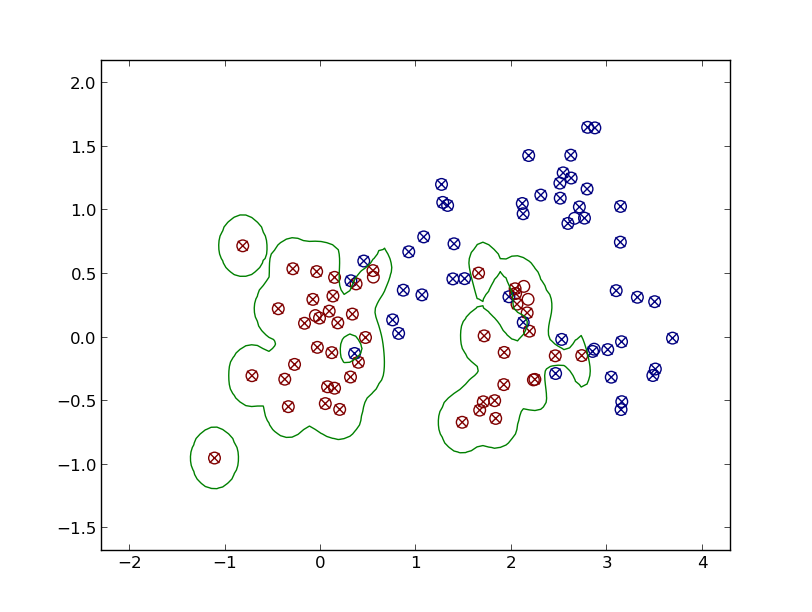
\includegraphics[width=6cm]{images/smallSigma.png}
			\end{figure}
			\begin{itemize}
				\item Small sigma
			\end{itemize}
		\end{column}
		\begin{column}{6cm}
			\begin{figure}
				\centering
				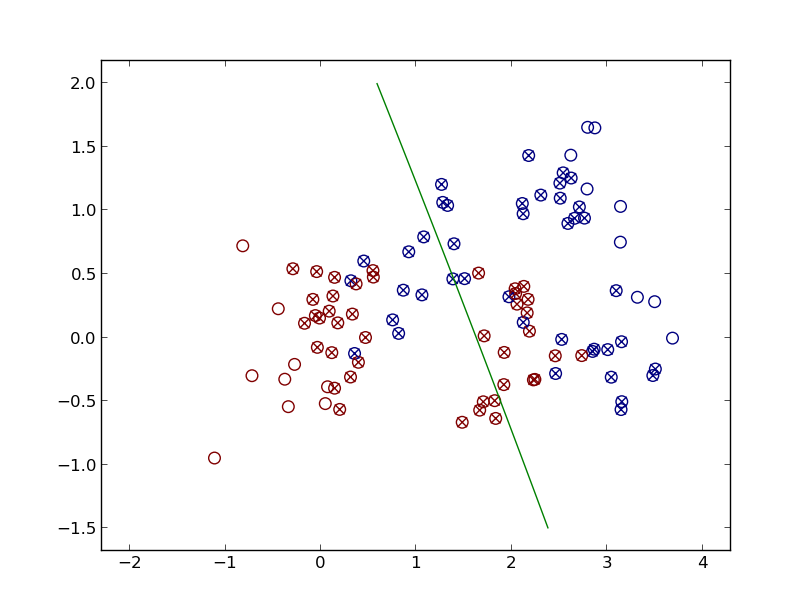
\includegraphics[width=6cm]{images/largeSigma.png}
			\end{figure}
			\begin{itemize}
				\item Large sigma
			\end{itemize}
		\end{column}
	\end{columns}
\end{frame}

\begin{frame}
	\frametitle{Locality}
	\begin{theorem}
		For the Gaussian kernel classifier, the normal of the tangent of the decision surface at $x$ is constrained to approximately lie in the pan of the vectors $(x-x_i)$ with $\norm{x-x_i}$ not large compared to $\sigma$ and $x_i$ in the training set.
	\end{theorem}
	
	Proof sketch:
	\begin{eqnarray*}
		\nabla_{\mathbf{x}}f(\mathbf{x}) &=& \nabla_{\mathbf{x}} \left( b + \sum_{i} \alpha_i K(\mathbf{x},\mathbf{x}_i) \right)\\
		&=& -\sum_{i} \alpha_i \frac{\norm{\mathbf{x}-\mathbf{x}_i}}{\sigma^2}K(\mathbf{x},\mathbf{x}_i)
	\end{eqnarray*}
	
	\begin{itemize}
		\item For $\mathbf{x}$ far away from $\mathbf{x}_i$, $K(\mathbf{x},\mathbf{x}_i)\approx 0$
		\item Vector dominated by $(\mathbf{x}-\mathbf{x}_i)$ with $\mathbf{x}_i$ being close to $\mathbf{x}$
	\end{itemize}
\end{frame}

\begin{frame}
	\frametitle{Implications}
	\begin{itemize}
		\item Tangent plane correctly determined iff number neighbours $>$ dimension of manifold
		\item Highly varying function requires small $\sigma$
		\item $\downarrow$ $\sigma$ $\Rightarrow$ $\downarrow$ number neighbours
		\item $\Rightarrow$ more training data points required
	\end{itemize}
\end{frame}

\begin{frame}
	\frametitle{Exponentially many training data points}
	\begin{itemize}
		\item Potentially exponentially many (w.r.t. the dimension) training data points required
		\item Due to locality, define ball around $x$ containing dominating neighbours
		\item Let $N$ be the number of these balls to cover the region $\Omega$
		\item Let $k$ be the smallest number of examples to reach error level $\epsilon$
		\item Thus, $k\cdot N$ training data points required
		\item Let $R$ be the radius of $\Omega$, then $O\left(\left(\frac{R}{r}\right)^d\right)$ radius-$r$ balls fit in $\Omega$
	\end{itemize}
\end{frame}
